%To compile as handout, use
%pdflatex "\def\ishandout{1} \input{filename.tex}"
%Defaults to non-handout mode (with slide reveals)
\ifdefined\ishandout
  \documentclass[handout]{beamer}
\else
  \documentclass{beamer}
\fi
 
\usepackage{econ103slides} 

\date{Lecture \# 11}
\begin{document} 

%%%%%%%%%%%%%%%%%%%%%%%%%%%%%%%%%%%%%%%%

\begin{frame}[plain]
	\titlepage 
	

\end{frame} 

%%%%%%%%%%%%%%%%%%%%%%%%%%%%%%%%%%%%%%%%


\begin{frame}

\centering \Huge Continuous RVs -- Part I

\end{frame}
%%%%%%%%%%%%%%%%%%%%%%%%%%%%%%%%%%%%%%%%

\begin{frame}
\frametitle{What Changes?}
	\begin{enumerate}
\item Probability Density Functions replace Probability Mass Functions (aka Probability Distributions)
\item Integrals Replace Sums
\end{enumerate}
\begin{alertblock}{Everything Else is Essentially Unchanged!}\end{alertblock}


\end{frame}

%%%%%%%%%%%%%%%%%%%%%%%%%%%%%%%%%%%%%%%%


\begin{frame}
\frametitle{What is the probability of ``Yellow?''\hfill 
\includegraphics[scale = 0.05]{./images/clicker}}
\centering
	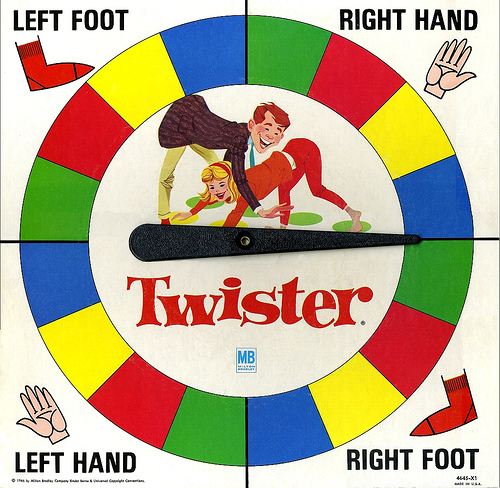
\includegraphics[scale = 0.6]{./images/twister}

\end{frame}
%%%%%%%%%%%%%%%%%%%%%%%%%%%%%%%%%%%%%%%%


\begin{frame}
\frametitle{What is the probability of ``Right Hand Blue?'' \hfill 
\includegraphics[scale = 0.05]{./images/clicker}}
\centering
	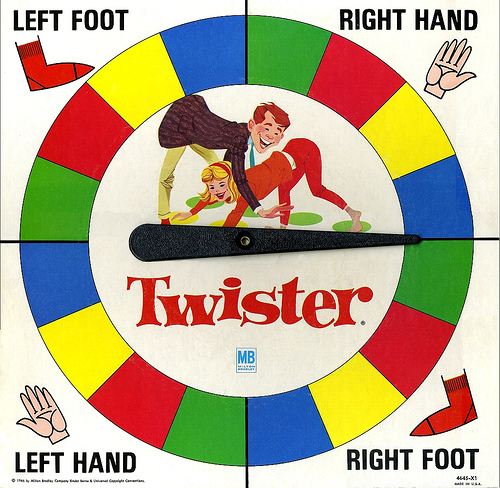
\includegraphics[scale = 0.6]{./images/twister}

\end{frame}
%%%%%%%%%%%%%%%%%%%%%%%%%%%%%%%%%%%%%%%%
\begin{frame}
\frametitle{What is the probability that the spinner lands in any \emph{particular} place?\hfill 
\includegraphics[scale = 0.05]{./images/clicker}}

\begin{center}
	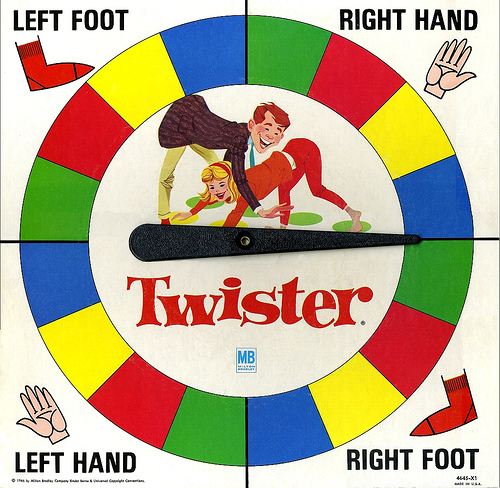
\includegraphics[scale = 0.6]{./images/twister}
\end{center}
\end{frame}




%%%%%%%%%%%%%%%%%%%%%%%%%%%%%%%%%%%%%%%%

\begin{frame}
\frametitle{From Twister to Density -- Probability as \emph{Area}}

\centering
	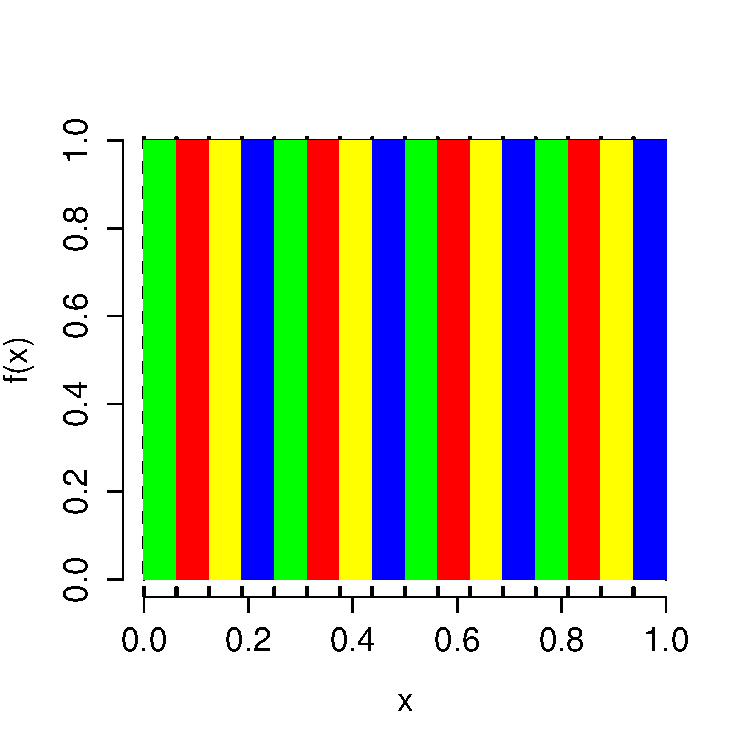
\includegraphics[scale = 0.6]{./images/twister_density}

\end{frame}


%%%%%%%%%%%%%%%%%%%%%%%%%%%%%%%%%%%%%%%%

\begin{frame}
\frametitle{Continuous Random Variables}

For continuous RVs, probability is a matter of finding the area of \emph{intervals}. Individual \emph{points} have \emph{zero} probability.

\end{frame}




%%%%%%%%%%%%%%%%%%%%%%%%%%%%%%%%%%%%%%%%

\begin{frame}
\frametitle{Probability Density Function (PDF)}
For a continuous random variable $X$, 
	$$P(a \leq X \leq b) = \int_a^b f(x) \; dx$$
where $f(x)$ is the \emph{probability density function} for $X$. 
\vspace{2em}

\begin{alertblock}{Extremely Important}
For any realization $x$, $P(X=x) = 0 \neq f(x)$!
\end{alertblock}
\end{frame}
%%%%%%%%%%%%%%%%%%%%%%%%%%%%%%%%%%%%%%%%
\begin{frame}
\frametitle{Properties of PDFs}
\begin{enumerate}
\item $\int_{-\infty}^\infty f(x) \; dx = 1$ 
\item $f(x) \geq 0$ for all $x$
\item $f(x)$ is \emph{not} a probability and can be greater than one!
\item $P(X\leq x_0) = F(x_0) = \int_{-\infty}^{x_0} f(x) \; dx $
\end{enumerate}
\end{frame}
%%%%%%%%%%%%%%%%%%%%%%%%%%%%%%%%%%%%%%%%
\begin{frame}
	\begin{center}
	\huge
		We'll start with the simplest possible example: the Uniform$(0,1)$ RV.
	\end{center} 
\end{frame}


%%%%%%%%%%%%%%%%%%%%%%%%%%%%%%%%%%%%%%%%
\begin{frame}
\frametitle{Uniform$(0,1)$ Random Variable}

\begin{block}{$X \sim \mbox{Uniform}(0,1)$}
We say that $X$ follows a Uniform(0,1) distribution, if it is equally likely to take on \emph{any value} in the range $[0,1]$ and never takes on a value outside this range.
\end{block}

\begin{block}{Uniform PDF}
$f(x) = 1$ for $0\leq x \leq 1$, zero elsewhere.
\end{block}

\end{frame}
%%%%%%%%%%%%%%%%%%%%%%%%%%%%%%%%%%%%%%%%


\begin{frame}
\frametitle{Uniform$(0,1)$ PDF}
\centering
	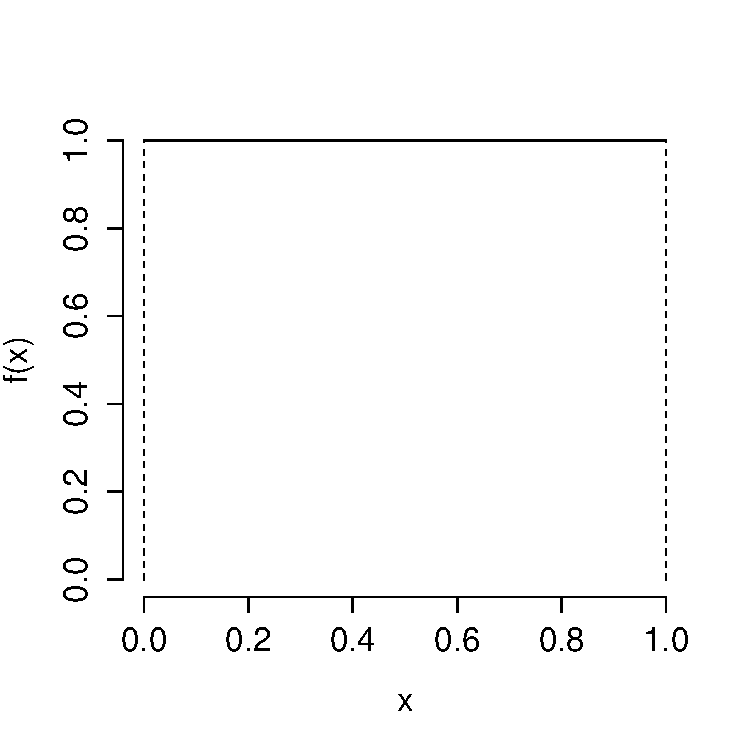
\includegraphics[scale = 0.6]{./images/uniform_density}

\end{frame}


%%%%%%%%%%%%%%%%%%%%%%%%%%%%%%%%%%%%%%%%
\begin{frame}
\frametitle{What is the area of the shaded region? \hfill 
\includegraphics[scale = 0.05]{./images/clicker}}

\centering
	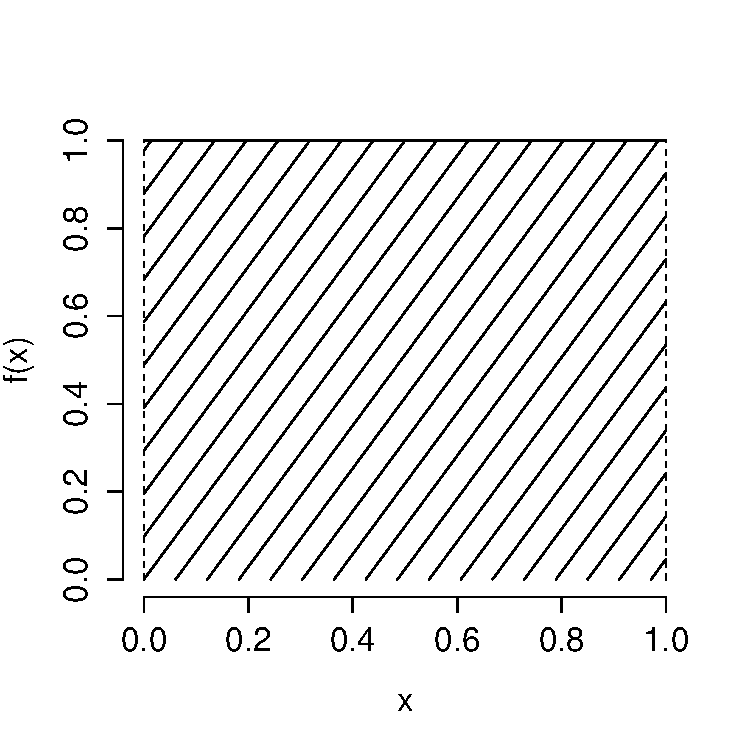
\includegraphics[scale = 0.6]{./images/uniform_density_shaded}

\end{frame}


%%%%%%%%%%%%%%%%%%%%%%%%%%%%%%%%%%%%%%%%

\begin{frame}
\frametitle{What is the area of the shaded region?}

\centering
	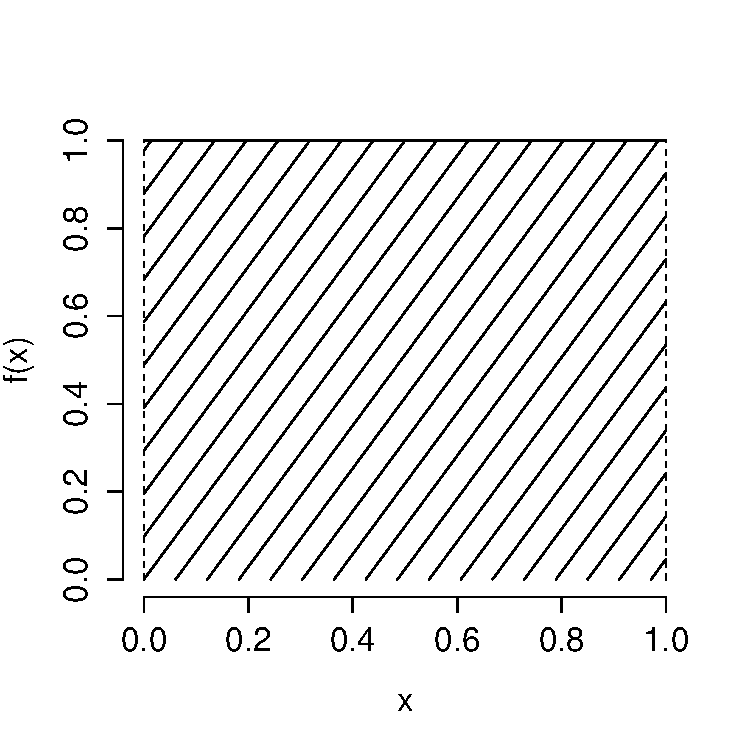
\includegraphics[scale = 0.4]{./images/uniform_density_shaded}
\begin{eqnarray*}
	\int_{-\infty}^{\infty} f(x) \; dx =\pause\int_{0}^1 1 \; dx = \pause \left. x \right|_0^1 =\pause 1 - 0 = 1
\end{eqnarray*}
\end{frame}


%%%%%%%%%%%%%%%%%%%%%%%%%%%%%%%%%%%%%%%%



\begin{frame}
\frametitle{What is the area of the shaded region? \hfill 
\includegraphics[scale = 0.05]{./images/clicker}}
\centering
	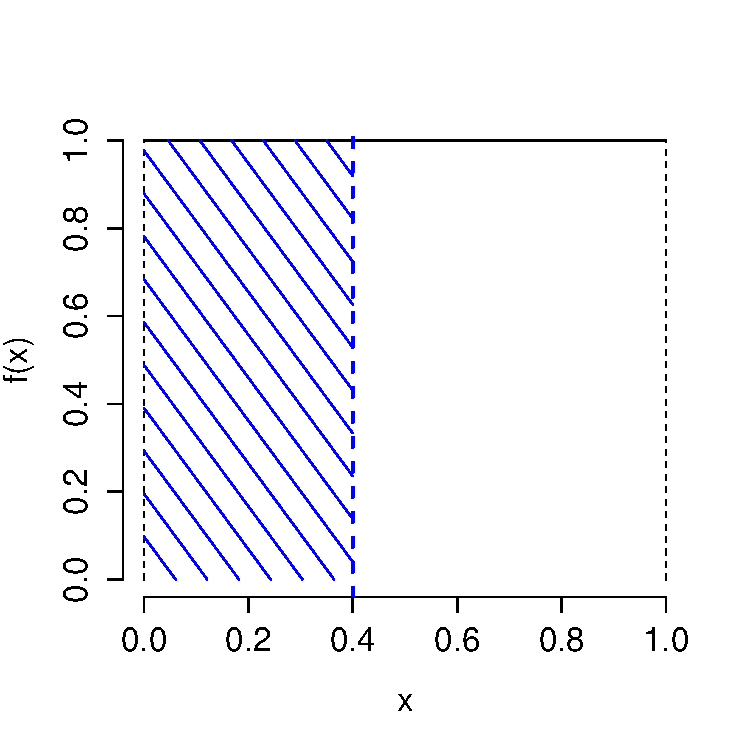
\includegraphics[scale = 0.6]{./images/uniform_density_cdf}

\end{frame}


%%%%%%%%%%%%%%%%%%%%%%%%%%%%%%%%%%%%%%%%

\begin{frame}
\frametitle{$F(0.4) = P(X\leq 0.4) = 0.4$}
\centering
	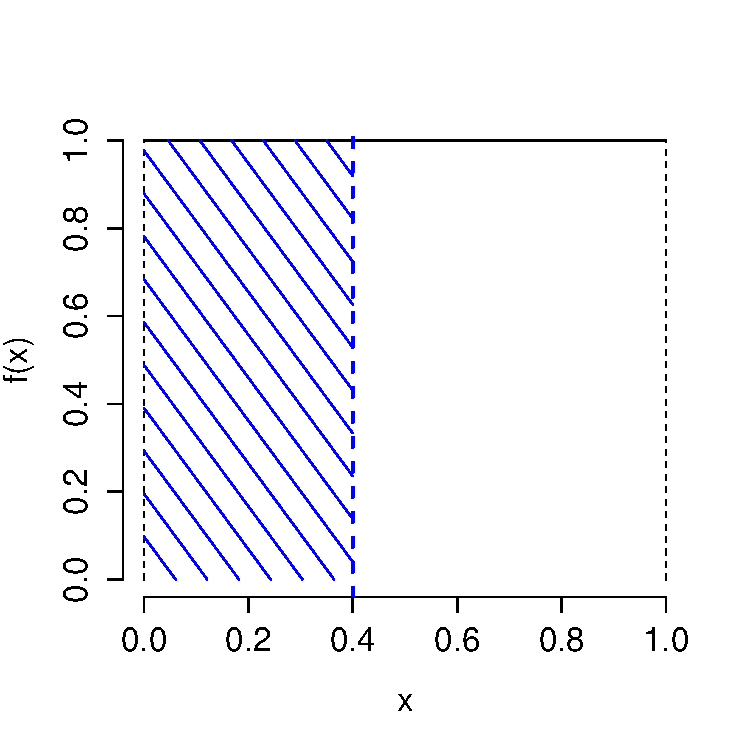
\includegraphics[scale = 0.6]{./images/uniform_density_cdf}

\end{frame}


%%%%%%%%%%%%%%%%%%%%%%%%%%%%%%%%%%%%%%%%


\begin{frame}
\frametitle{Relationship between PDF and CDF}

Integrate the pdf to get the CDF
	$$F(x_0) = P(X\leq x_0) = \int_{-\infty}^{x_0} f(x)\; dx$$
Differentiate the CDF to get the pdf
 	$$f(x) =\frac{d}{dx}F(x)$$
\alert{This is just the Fundamental Theorem of Calculus.}
\end{frame}


%%%%%%%%%%%%%%%%%%%%%%%%%%%%%%%%%%%%%%%%
\begin{frame}
\frametitle{Example: Uniform$(0,1)$ RV}

Integrate the pdf, $f(x) = 1$, to get the CDF
\begin{eqnarray*}
	F(x_0) =\int_{-\infty}^{x_0} f(x)\; dx =\pause \int_{0}^{x_0} 1\; dx = \pause \left. x \right|_0^{x_0} =\pause x_0 - 0 = x_0
\end{eqnarray*}

\vspace{1em}
$$ F(x_0) = \left\{ \begin{array}{c} 0, x_0 < 0\\ x_0, 0\leq x_0 \leq 1\\ 1, x_0 > 1   \end{array}\right.$$
\end{frame}


%%%%%%%%%%%%%%%%%%%%%%%%%%%%%%%%%%%%%%%%
\begin{frame}
\frametitle{Uniform$(0,1)$ CDF}
\centering
	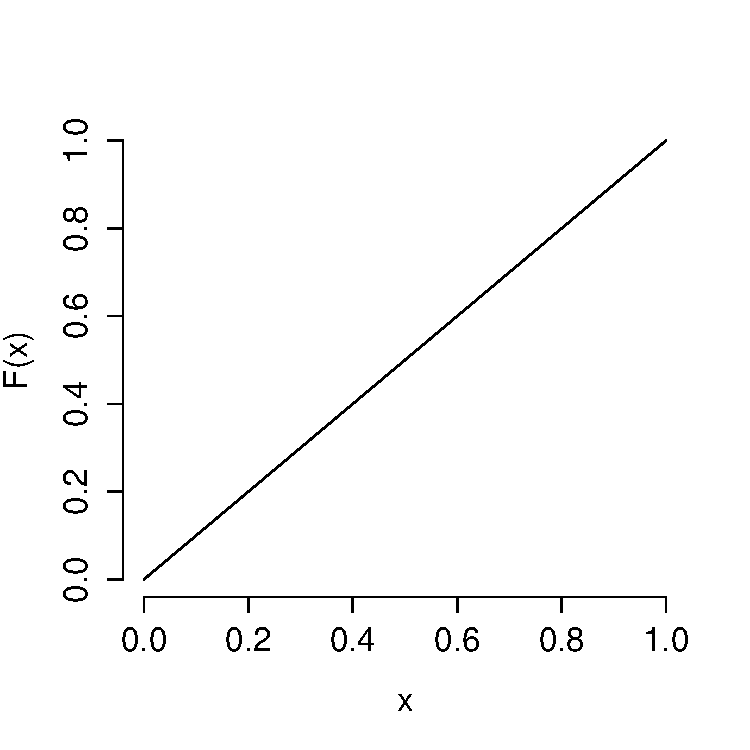
\includegraphics[scale = 0.6]{./images/uniform_CDF}

\end{frame}


%%%%%%%%%%%%%%%%%%%%%%%%%%%%%%%%%%%%%%%%
\begin{frame}
\frametitle{Example: Uniform$(0,1)$ RV}
Differentiate the CDF, $F(x_0) = x_0$, to get the pdf
 \begin{eqnarray*}
	\frac{d}{dx}F(x) =  1 = f(x)
 \end{eqnarray*}
\end{frame}



%%%%%%%%%%%%%%%%%%%%%%%%%%%%%%%%%%%%%%%%

\begin{frame}
\Huge \begin{center}Key Idea: Probability of Intervals\end{center}
\end{frame}
%%%%%%%%%%%%%%%%%%%%%%%%%%%%%%%%%%%%%%%%
\begin{frame}
\frametitle{What is $P(0.4 \leq X \leq 0.8)$ if $X\sim \mbox{Uniform}(0,1)$? \hfill 
\includegraphics[scale = 0.05]{./images/clicker}}
\centering
	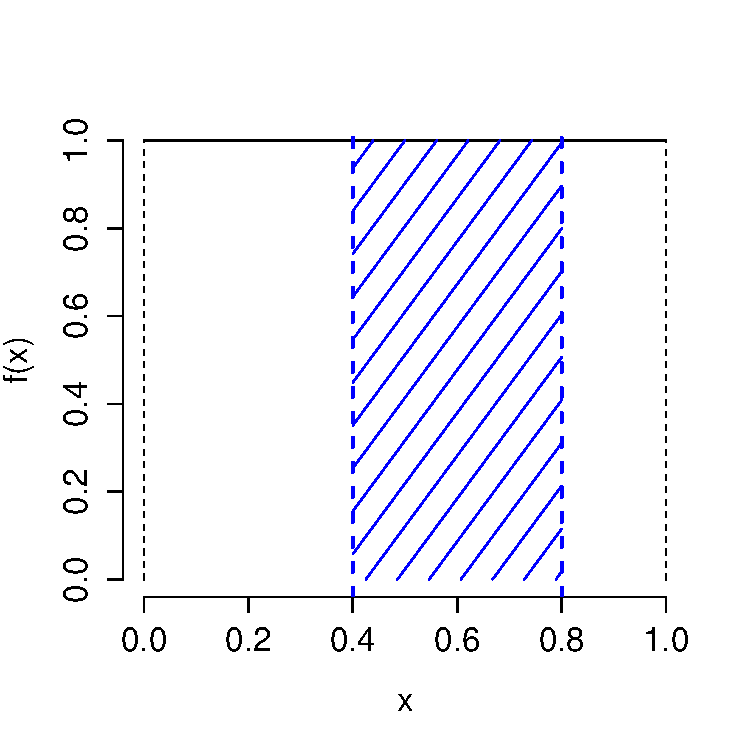
\includegraphics[scale = 0.6]{./images/uniform_density_interval}


\end{frame}
%%%%%%%%%%%%%%%%%%%%%%%%%%%%%%%%%%%%%%%%
\begin{frame}
\frametitle{$F(0.8) = P(X \leq 0.8)$}

\centering
	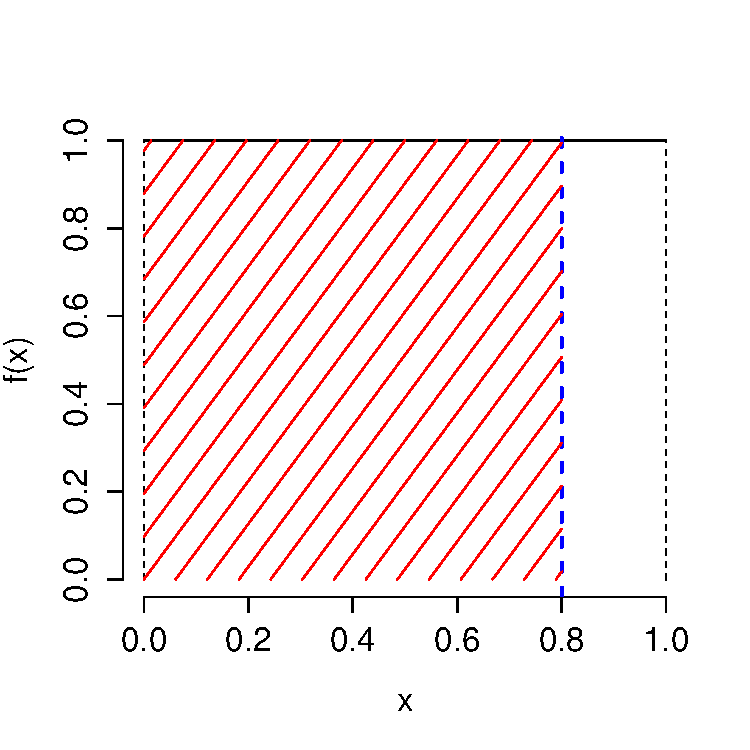
\includegraphics[scale = 0.6]{./images/density_interval_cdf1}

\end{frame}


%%%%%%%%%%%%%%%%%%%%%%%%%%%%%%%%%%%%%%%%
\begin{frame}
\frametitle{$F(0.8) - F(0.4) = $ ?}
\centering
	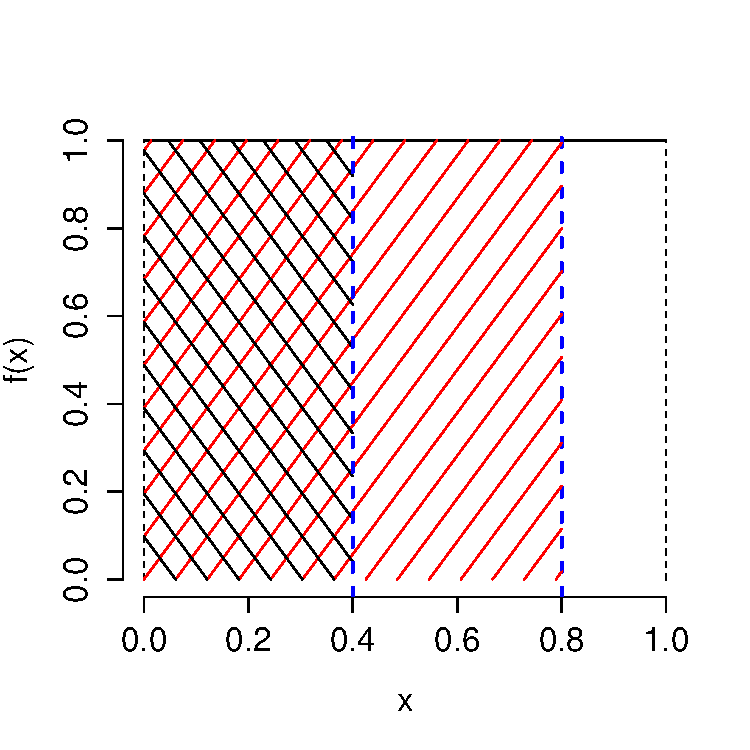
\includegraphics[scale = 0.6]{./images/density_interval_cdf2}

\end{frame}


%%%%%%%%%%%%%%%%%%%%%%%%%%%%%%%%%%%%%%%%
\begin{frame}
\frametitle{$F(0.8) - F(0.4) = P(0.4 \leq X \leq 0.8) = 0.4$}
\centering
	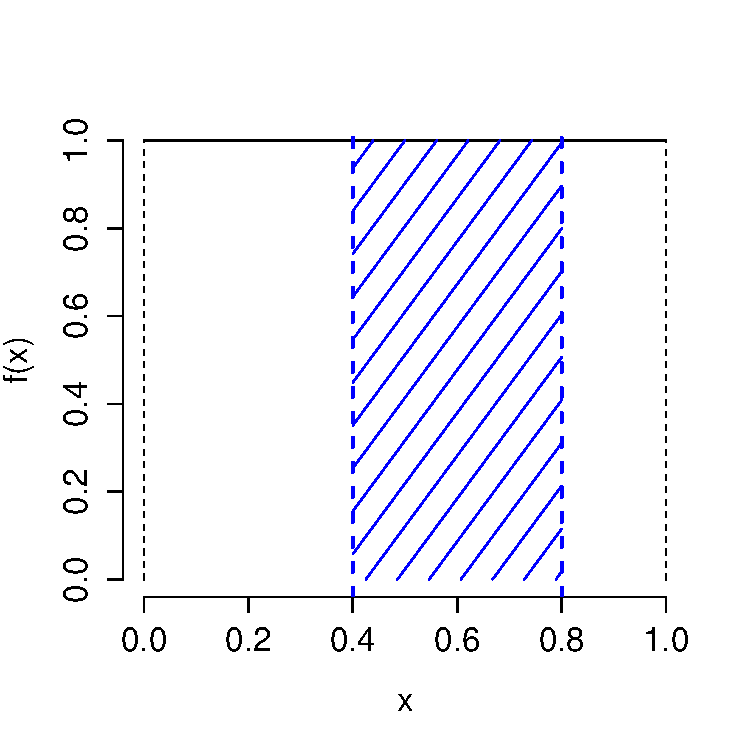
\includegraphics[scale = 0.6]{./images/uniform_density_interval}


\end{frame}
%%%%%%%%%%%%%%%%%%%%%%%%%%%%%%%%%%%%%%%%
\begin{frame}
\frametitle{Probability of Interval for Continuous RV}

$$\boxed{P(a\leq X \leq b) = \int_a^b f(x) \; dx = F(b) - F(a)}$$

\vspace{2em}
\alert{This is just the Second Fundamental Theorem of Calculus.}
\end{frame}
%%%%%%%%%%%%%%%%%%%%%%%%%%%%%%%%%%%%%%%%

\begin{frame}
\frametitle{Expected Value for Continuous RVs}
$$\boxed{\int_{-\infty}^\infty x f(x) \; dx  }$$

\vspace{2em}
\alert{Remember: Integrals Replace Sums!}
\end{frame}

%%%%%%%%%%%%%%%%%%%%%%%%%%%%%%%%%%%%%%%%
\begin{frame}
\frametitle{Example: Uniform(0,1) Random Variable \hfill 
\includegraphics[scale = 0.05]{./images/clicker}}
\begin{eqnarray*}
	E[X] &=&  \int_{-\infty}^\infty x f(x) \; dx =\pause  \int_{0}^1 x \cdot 1 \; dx \\ \\
		&=&  \left.\frac{x^2}{2}\right|_0^1 = 1/2  - 0 = 1/2
\end{eqnarray*}
\end{frame}
%%%%%%%%%%%%%%%%%%%%%%%%%%%%%%%%%%%%%%%%
\begin{frame}
\frametitle{Expected Value of a Function of a Continuous RV}
	$$\boxed{E[g(X)] = \int_{-\infty}^\infty g(x) f(x) \; dx}$$
\end{frame}


%%%%%%%%%%%%%%%%%%%%%%%%%%%%%%%%%%%%%%%%

\begin{frame}
\frametitle{Example: Uniform$(0,1)$ RV}
	\begin{eqnarray*}
	E[X^2] &=& \int_{-\infty}^\infty x^2 f(x) \; dx = \int_0^1 x^2 \cdot 1 \; dx\\ \\
		&=& \left. \frac{x^3}{3}\right|_0^1 = 1/3
	\end{eqnarray*}
\end{frame}


%%%%%%%%%%%%%%%%%%%%%%%%%%%%%%%%%%%%%%%%

\begin{frame}
Once we have defined expected value for continuous RVs, we can use everything we know about variance, covariance, etc.\ from discrete RVs!
\end{frame}

%%%%%%%%%%%%%%%%%%%%%%%%%%%%%%%%%%%%%%%%
\begin{frame}
\frametitle{Variance of Continuous RV}

$$\boxed{Var(X) = \int_{-\infty}^{\infty} (x - \mu)^2 f(x) \; dx}$$

\vspace{2em}
where
$$\mu = E[X]=\int_{-\infty}^\infty x f(x) \; dx $$

\vspace{2em}
\alert{Shortcut formula still holds for continuous RVs!}
	$$Var(X) = E[X^2] - \left(E[X]\right)^2$$
\end{frame}
%%%%%%%%%%%%%%%%%%%%%%%%%%%%%%%%%%%%%%%%

\begin{frame}
\frametitle{Example: Uniform(0,1) Random Variable \hfill 
\includegraphics[scale = 0.05]{./images/clicker}}
\begin{eqnarray*}
 Var(X) &=& E\left[ \left( X - E[X] \right)^2\right] = E[X^2] - \left(E[X]\right)^2\\ \pause
 	&=& 1/3  - (1/2)^2\\ 
 	&=& 1/12 \\
 	&\approx& 0.083
\end{eqnarray*}
\end{frame}

%%%%%%%%%%%%%%%%%%%%%%%%%%%%%%%%%%%%%%%%
\begin{frame}
\frametitle{Much More Complicated Without the Shortcut Formula!}
\begin{eqnarray*}
 Var(X) &=& E\left[ \left( X - E[X] \right)^2\right] = \int_{-\infty}^{\infty} (x - \mu)^2 f(x) \; dx\\ \\
 	&=&\int_{0}^{1} (x -1/2)^2 \cdot 1 \; dx = \int_{0}^{1} (x^2  - x + 1/4) \; dx \\ \\
 		&=& \left. \left(\frac{x^3}{3} - \frac{x^2}{2} + \frac{x}{4}  \right)\right|_0^1 = 1/3 - 1/2 + 1/4\\ \\ 
 			&=& 4/12 - 6/12 + 3/12 = 1/12
\end{eqnarray*}
\end{frame}

%%%%%%%%%%%%%%%%%%%%%%%%%%%%%%%%%%%%%%%%
\begin{frame}
\frametitle{We're Won't Say More About These, But Just So You're Aware of Them...}

\begin{block}{Joint Density}
$ \displaystyle P(a\leq X \leq b \cap c\leq Y \leq d) = \int_c^d \int_a^b f(x,y) \; dxdy$
\end{block}
\begin{block}{Marginal Densities}
$f_X(x) = \int_{-\infty}^\infty f(x,y)\; dy$, $\;\;\;\;\;\;\; f_Y(y) = \int_{-\infty}^\infty f(x,y)\; dx$
\end{block}
\begin{block}{Independence in Terms of Joint and Marginal Densities}
$f_{XY}(x,y) = f_X(x)f_Y(y)$
\end{block}
\begin{block}{Conditional Density}
$f_{Y|X} = f_{XY}(x,y)/f_X(x)$
\end{block}

\end{frame}

%%%%%%%%%%%%%%%%%%%%%%%%%%%%%%%%%%%%%%%%
\begin{frame}

\huge We've now covered everything on the \href{http://ditraglia.com/Econ103Public/RandomVariablesHandout.pdf}{\textcolor{blue}{\fbox{Random Variables Handout}}}

\end{frame}
%%%%%%%%%%%%%%%%%%%%%%%%%%%%%%%%%%%%%%%%

\end{document}
